\documentclass[authoryear,preprint,review,12pt]{elsarticle}
\usepackage[utf8x]{inputenc}
\usepackage[a4paper, total={6.5in, 10.5in}]{geometry}
\usepackage[round]{natbib}
\bibliographystyle{plainnat}
\usepackage{filecontents}
\usepackage{lscape}
\usepackage{lipsum}
\usepackage{booktabs}
\usepackage{tabularx}
\usepackage{tablefootnote}
\usepackage{threeparttable}
\usepackage{caption}
\usepackage{subcaption}
\usepackage [autostyle, english = american]{csquotes}
\MakeOuterQuote{"}
\captionsetup[figure]{font=footnotesize}
\captionsetup[table]{font=footnotesize}
\usepackage{rotating}
\usepackage{adjustbox}
\usepackage{graphicx}
\usepackage{amsmath}
\usepackage{hyperref}
\usepackage{setspace}
\usepackage{float}
\usepackage{array}
\usepackage{csvsimple}
\usepackage{threeparttable}
\setlength{\tabcolsep}{9pt}
\renewcommand{\arraystretch}{1.2}
\usepackage{pgfplotstable}
\pgfplotsset{compat=1.18}
\usepackage{array, multirow,makecell}
\newcolumntype{R}[1]{>{\raggedleft\arraybackslash }b{#1}}
\newcolumntype{L}[1]{>{\raggedright\arraybackslash }b{#1}}
\newcolumntype{C}[1]{>{\centering\arraybackslash }b{#1}}
\usepackage{wrapfig, blindtext}
\usepackage{booktabs} % For \toprule, \midrule and \bottomrule
\usepackage{siunitx} % Formats the units and values
\hypersetup{colorlinks=true,
    linkcolor=blue,
    filecolor=blue,      
    urlcolor=blue,
    citecolor=blue
    }
\urlstyle{same}
\onehalfspacing
\usepackage{graphicx}
\graphicspath{ {./images/}}


\journal{GRASS workshop 2024}

\begin{document}


\begin{frontmatter}


\title{Asylum seekers integration and local public finances: evidence from Italian refugees reception centres}
\author[inst1]{Matteo Caruso}
\author[inst2]{Giuseppe Migali}
\affiliation[inst1]{organization={Department of Economics, Lancaster University Management School, Lancaster University},
             city={Lancaster},
             postcode={LA1 4YX},
             country={UK}}
\affiliation[inst2]{organization={Department of Economics, Law, and Sociology, Magna Graecia University}, city={Catanzaro},  country={Italy}}
 \date{}




\begin{abstract}

 THIS IS A PRELIMINARY AND INCOMPLETE VERSION - DO NOT CITE
 \\
 
 \vspace{10}
 
\noindent
This paper studies the impact of the presence of Italian Asylum Seeker Reception Centres (ASRC), also called SPRAR, on municipalities' public finances.\ These centres are secondary hosting to provide the refugees with job formation, educational activities, and language courses.\ Using municipality-level data from 2005 to 2014, our main findings show that the presence of one SPRAR does not increase the overall expenditure of the local municipality but it affects its composition, with a substantial increase in public expenditure on social activities around 3\%.\ The effect remains significant when controlling for demographic and political variables.\ Most of the projects involve small municipalities with less than 5000 citizens, so the presence of the reception facility may provide a great impact on the local community and welfare activities.\\ 
\end{abstract}


\begin{keyword}
Asylum seekers reception centres \sep public finances \sep education \sep migration \sep local investments

\JEL K37 \sep H52 \sep H71 \sep H72 \sep 015
\end{keyword}



\end{frontmatter}

\section{Introduction}

\noindent
The problem of refugees has been a hot topic within the European Union for many years, especially for the Mediterranean countries, such as Italy, Greece, and Spain.\ The global political scenario in the past decades has been strongly influenced by the problem of illegal migration, both in the U.S. and Europe \citep{bracco2018}.\ Italy, for its strategic position, has been for several years at the centre of this debate, for being often 'the first country of entry', receiving most of the refugees from North Africa.\ In 2017, Italy was the second EU country, after Germany, for the number of asylum applications \citep{campesi2018}.\ Part of the problem has been exacerbated by the 'hotspot approach' adopted by the EU, for which detention centres were created to identify asylum seekers and process their applications.\ According to \cite{campesi2018}, it is possible to divide the reception system for asylum seekers into two categories: 'first' and 'second' reception, a division strongly incentivised by the UNHCR too.\ While the first reception centres, so-called 'hotspots', have a logic of 'containment' into large and crowded centres, the latter focuses on 'dispersal' action, allocating refugees in small-size reception facilities, most of the time provided by the private sector \citep{campesi2018}.\ This second approach comes from the idea that refugees are better suited to be integrated while being in a smaller community, avoiding the risk of segregation in larger and more crowded metropolitan areas.\ While implemented informally by local authorities and NGOs at the end of the 1990s, this system has been institutionalised through the creation of a Protection System for Asylum Seekers and Refugees (SPRAR) in which those small and medium facilities are framed.\ Although smaller in terms of the number of refugees, we focus on the second type of reception, which provides different type of projects for the refugee, often focusing on job formation and social activity within the community.\\

\noindent
SPRAR centers had been legally introduced with Law n°189/2002, establishing a National Asylum Programme (PNA), with the purpose of dealing with the increasing number of refugees coming to the country \citep{cittalia2022}.\ To fund these projects, the Ministry of the Interior has established a "Fund for Asylum Policies and Services" which covers up to 95\% of the cost of the SPRAR \citep{ricardguay2019}.\ A substantial part of the revenues financing the project comes therefore from the central government.\ While the municipality is the one applying to the Ministry of the Interior to open the hosting facility, it is not the one receiving the financial contribution.\ The majority of the projects are actually managed and organised by the entities from the third sectors, i.e.\ NGOs with different social purposes.\ The municipality has the role to overlook and control the correct proceeding of the project, but most of the revenues from the fund goes to the NGO managing the activities \citep{ricardguay2019}.\ Given the absence of direct financial contributions from the central government, we therefore explore the presence of eventual indirect effects of these projects on municipalities' public finances, analysing the composition of their expenditures.\\ 

\noindent
Using municipality-level data for a period of ten years, from 2005 to 2014, we find that the presence of a SPRAR facility in the community does not significantly affect the size of local public expenditure of the interested municipality.\ Nonetheless, when decomposing the total expenditure, the share of public expenditure dedicated to social activities substantially increases in the treated units.\ Such effect remain significant when controlling for the municipality's population and its political affiliation.\ We also control for any public revenues coming from the government, excluding any possible direct contribution from the Ministry of the Interior.\ The main thesis is that, given the presence of the reception facility, the local authority devolves more attention to the organisation of social activities related to the project, compared to other sectors, such as transportation or infrastructure.\ We do not see any relevant change in the share of expenditure addressed to other activities though.\ While it is not clear what direct effect these project have on the overall community, they have indeed a relevant role in the structure of the local government, with eventual both positive and negative spillovers.\\ 


\noindent
Several papers have tried to explore what are the main effects of migration on local public finances.\ \cite{gerdes2011} explores the hypothesis that ethnically heterogeneous Danish cities are correlated with a smaller public size of the local government but finds no presence of this correlation over time, after a relevant surge in the number of incoming refugees in Denmark, between 1995 and 2001.\ \cite{senses2022} found out instead that an increase in the total share of immigrants in U.S.\ counties does not affect local public revenues or expenditures.\ Nonetheless, when dividing between high-skilled and low-skilled, the former group seems to have a positive impact on both local revenues and expenditure, while low-skilled immigrants have instead the opposite effect.\ Nonetheless, voluntary migration is different from a forced one, as is the case of asylum seekers.\ The needs and contributions of both groups might differ substantially, and so they could have different effects on local governments.\ Closer to our research, \cite{chevalier2023} study the effects of force migration on public policy in post-war West Germany.\ Cities that witnessed a higher number of forced migrants increased their expenditures on welfare and education, reducing instead those on infrastructure and raising local taxes.\ Our work moves in the same direction, providing evidence that those projects involving the integration of refugees, through job allocation programmes, training, and language courses, may improve the fiscal health of the local government.\ 


\vspace{5}

\section{Data and identification strategy}
\noindent
In this paper, we focus on Italian municipalities and the presence of an Asylum Seeker Reception Centre (ASRC) in Italy, defined as Protection System for Asylum Seekers and Refugees (SPRAR).\ We build on the dataset from \cite{proietti2022} \footnote{We are grateful to Davide Luca for providing us with the data}, where they use a novel dataset to find a correlation between the presence of SPRAR and organised crime in Italy in 2016.\ While they had data for SPRAR centres in 2010 and between 2012 and 2016, we managed to integrate their dataset with information from the single reports, managing to create a dummy for the municipalities with a SPRAR centre from 2005 to 2009 \citep{cittalia2022}.\ Since we do not use the actual number of refugees but a simple dummy to assess the presence of one ASRC, we infer the values for 2011 with the assumption that if a municipality had one centre in 2010 and in 2012, the same centre remained open in 2011 as well.\ \citep{cittalia2022}.\\ 

\noindent
 Data on local public finances come instead from the website of the Open Polis Foundation, collecting data for each single Italian municipality from 2005 to 2020 \citep{openpolis2024}.\ Due to a legal reform that changed the modality of collection of the data for municipalities, we have been able to work on local finances only from 2005 to 2014.\ Moreover, since 2015, new legislation enhanced the creation of Extraordinary Emergency Centres (CAS) in many Italian municipalities \citep{ricardguay2019}.\ These are first-line reception facilities which have been established to face the growing number of arrivals from North Africa in those years.\ Given the different nature and purpose of such centres, their presence is likely to bias the direct effect of SPRARs in our study.\ Thus, we limit the analysis to the period before the introduction of this new legislation.\ A more exhaustive analysis covering the post-CAS scenario is left for future research.\\

 \noindent
 Using data on municipalities' elected representatives from the Ministry of the Interior, we also control for the political affiliation of each municipality.\ The data provides also information on the municipality's population, that we use as control as well \citep{ministerointerno}.\ We use each mayor's political affiliation or the composition of the coalition that supports them.\ If the mayor is not present, we use the vice-mayor's supporting coalition.\ When both are not present, we define the municipality's political orientation through a simple majority of the other elected representatives (i.e.\ assessori).\ Given the wide range of different local parties present in municipalities' elections, we simplify the affiliation in five categories, depending on the coalitions: left, center-left, center, center-right, right, and independent.\ Other studies have established a correlation between anti-immigration policies and far-right or conservative parties \citep{bracco2018}, while left and more liberal coalitions are likely to promote such reception facilities.\ Controlling for the municipality's political affiliation help us reduce the possible endogenity in the presence of the SPRAR.\\ 

\noindent
 Another source of endogenity, involves both the status of the native and foreign population.\ Given the demographic shrinking of many small Italian municipalities, many mayors may have the interest of welcoming more refugees to slow the population decrease.\ On another note, the presence of a large number of foreign residents may also be a signal of a municipality's disposition to welcome foreigners into their community.\ We therefore use census data from the Italian National Office of Statistics (ISTAT), which provides data on both Italian and non-Italian residents in each municipality for any given year.\footnote{Freely available at: \url{https://demo.istat.it/app/?i=RCS&l=it}}\ Our results do not change even when controlling for these variables.\\

\section{Results}

\noindent
As a first step, we run a simple difference-in-difference using OLS (Table \ref{tab1}).\ Although very basic, they show how total expenditures do not seem to be correlated with the presence of the SPRAR (column 1).\ When looking at the share of expenditures dedicated to social activities, such as kindergarten, cemeteries, services to the elderly, etc, they increase by 2.95\% (column 2).\ No other significant results appear when running the analysis for education, transportation, or similar.\ Dividing further between those social activities, the only one showing significant results is the residual part, dedicated to solidarity or charity projects.\ It increases by more than 3\% (column 3).\\

\noindent
Since the standard DID approach does not consider the possibility of multiple treatments for different units, for our main analysis, we follow \cite{clarke2020} in their approach to event study with multiple treatments.\ To have a pre-treatment period also for the treated units, we limit the analysis to the units whose SPRAR was opened for the first time in 2008.\ In this manner, we have at least three years of data for the treated units before the opening of the facility.\ Using all periods or avoiding to use never treated as control (i.e.\ those municipalities that had no SPRAR centres between 2005 and 2014) does not change our main results, although standard errors may vary significantly.\\ 



\begin{table}[H]
    \centering
        \caption{OLS table for the analysis.\ Data are from the website \url{https://openbilanci.it/}, taken in logs}
{
\def\sym#1{\ifmmode^{#1}\else\(^{#1}\)\fi}
\fontsize{7.2}{7.2}\selectfont
\begin{tabular}{l*{3}{c}}
\hline\hline
            &\multicolumn{1}{c}{(1)}&\multicolumn{1}{c}{(2)}&\multicolumn{1}{c}{(3)}\\
            &\multicolumn{1}{c}{Total expenditure (log)}&\multicolumn{1}{c}{Social expenditure (share)}&\multicolumn{1}{c}{Residual social expenditure (share)}\\
\hline
SPRAR          &      0.0261         &      0.0295\sym{***}&      0.0308\sym{***}\\
            &      (1.66)         &      (5.89)         &      (7.69)         \\
[1em]
Total revenues (log)&      0.0239\sym{***}&     0.00472\sym{***}&     0.00354\sym{***}\\
            &     (10.65)         &      (6.62)         &      (6.23)         \\
[1em]
Center party/coalition      &     -0.0103         &     0.00656         &    -0.00335         \\
            &     (-0.63)         &      (1.27)         &     (-0.81)         \\
[1em]
Center-left party/coalition  &     -0.0142         &     0.00316         &    -0.00225         \\
            &     (-1.11)         &      (0.78)         &     (-0.70)         \\
[1em]
Center-right party/coalition&    -0.00887         &    0.000949         &    -0.00221         \\
            &     (-0.72)         &      (0.24)         &     (-0.71)         \\
[1em]
Independent party/coalition &    -0.00670         &     0.00395         &   -0.000831         \\
            &     (-0.58)         &      (1.07)         &     (-0.28)         \\
[1em]
Left party/coalition        &     0.00114         &     0.00389         &   -0.000425         \\
            &      (0.04)         &      (0.47)         &     (-0.06)         \\
[1em]
Population (log)      &       0.127\sym{***}&    -0.00260         &     -0.0104         \\
            &      (3.70)         &     (-0.24)         &     (-1.20)         \\
[1em]
African population (log)&    -0.00429         &     0.00362\sym{*}  &     0.00191         \\
            &     (-0.89)         &      (2.36)         &      (1.56)         \\
[1em]
Foreign population (log)&    0.000424         &    -0.00346         &    -0.00379\sym{*}  \\
            &      (0.06)         &     (-1.65)         &     (-2.26)         \\
[1em]
Constant      &       8.811\sym{***}&      0.0805         &       0.130         \\
            &     (32.60)         &      (0.94)         &      (1.90)         \\
\hline
\(N\)       &       10318         &       10318         &       10318         \\
\hline\hline
Municipality FE & Yes & Yes & Yes \\
Year FE & Yes & Yes & Yes \\ 
\hline\hline
\multicolumn{4}{l}{\footnotesize \textit{t} statistics in parentheses}\\
\multicolumn{4}{l}{\footnotesize \sym{*} \(p<0.05\), \sym{**} \(p<0.01\), \sym{***} \(p<0.001\)}\\
\end{tabular}
}

    \label{tab1}
\end{table}

\noindent
In the event study, the size of the results varies due to the absence of enough control groups in the last periods after the treatment, when only a few municipalities are yet to be treated compared to the previous years.\ The main results remain robust though, with total expenditure showing no significant variation in the years following the opening of the SPRAR (Figure \ref{fig1}).\ For what concerns the other expenditures, although only for the first year, they show significant positive results (Figure \ref{fig2} and \ref{fig3}), both showing an increase in the share of around 3\%.\ In all three scenarios, we use the same control variables as the ones in the DID approach.\\ 

\noindent
These findings corroborate our main idea that even when controlling for the municipality's revenues, avoiding any possible direct effect of the Ministry of the Interior's fund, the social expenditure increases in the first year of the opening of the facility.\ This change of priorities in local public finances may have multiple relevant spillovers: the active participation of the municipality in the reception center could help the integration of the refugees and provide better results for the projects, enhancing the multiple-level governance (MLG) approach which is at the core of the PNA.\ On the negative side, it may reduce other resources for different activities, such as education or public transport.\ This latter scenario seems rather unlikely though, given the other expenditures do not seem to show any variation in the opposite direction, suggesting a rather smaller reduction of different expenses, with no very significant effect overall.\\


\begin{figure}[H]
\begin{minipage}[t]{.5\linewidth}
   \centering
    \caption{Effect on total expenditure}
    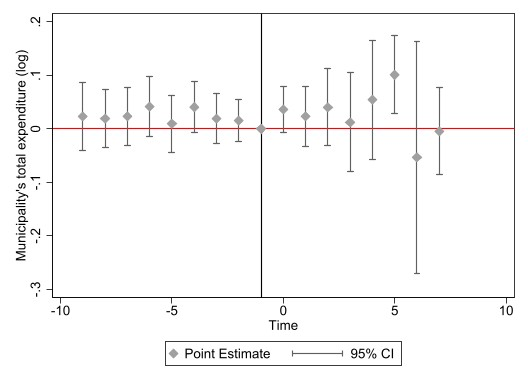
\includegraphics[scale = 0.5]{images/total event dd.jpg}
    \label{fig1}
\end{minipage}\hfill
\begin{minipage}[t]{.5\linewidth}
    \centering
    \caption{Effect on social services}
    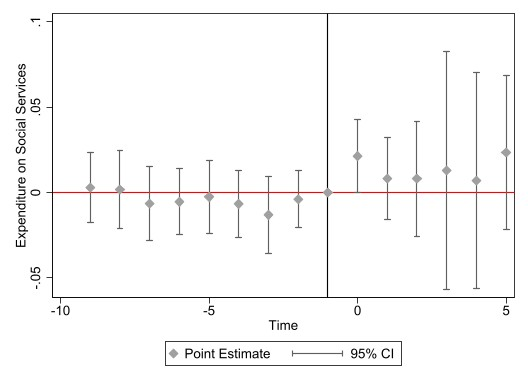
\includegraphics[scale = 0.5]{images/social event dd.jpg}
    \label{fig2}
\end{minipage}
    \centering
    \caption{Effect on charity and solidarity services}
    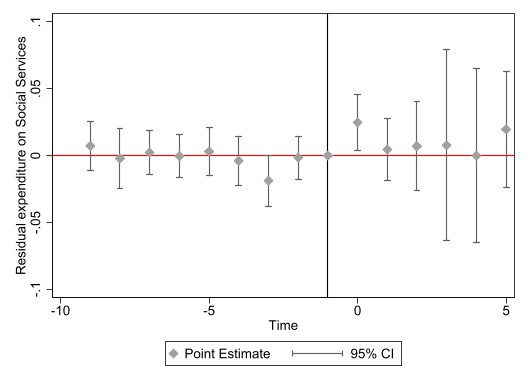
\includegraphics[scale = 0.5]{images/residual event dd.jpg}
\label{fig3}
\end{figure}


\section{Conclusion}

\noindent
Even considering its limitations, this work is the first paper to analyse the impact of second-hosting asylum seekers reception centres (SPRAR) on local public finances in Italy, whose final objective is the integration and the formation of the refugees, with relevant spillovers on the hosting municipality's fiscal expenditures and local investments in social activities.\\ 

\bibliography{references2}

\end{document}